\chapter{Resultater}
Resultatet af denne opgave er endt ud i en prototype af Child Security Systemet, dokumentationen af dette system, samt denne rapport omhandlende systemet.  

Igennem en velstruktureret arkitektur er det lykkedes at udarbejde et system som kan udføre de ønskede opgaver. Disse opgaver udføres af systemet dels gennem RS232 kommunikation mellem PC og STK500 og dels med X10-kommunikation mellem CSS-hovedenhed og X10-udtag. User-Interfacet har opnået flow som specificeret i arkitekturen. 
Prototypen er opbygget på veroboards, disse se på nedenstående figure \ref{fig:encoder_vero} og \ref{fig:decoder_vero}. Først er det udarbejdet printudlæg for hhv. encoder og decoder, disse er herefter produceret i loddelab. 

\begin{figure}[htb]
  \begin{minipage}{0.5\textwidth}
    \centering
      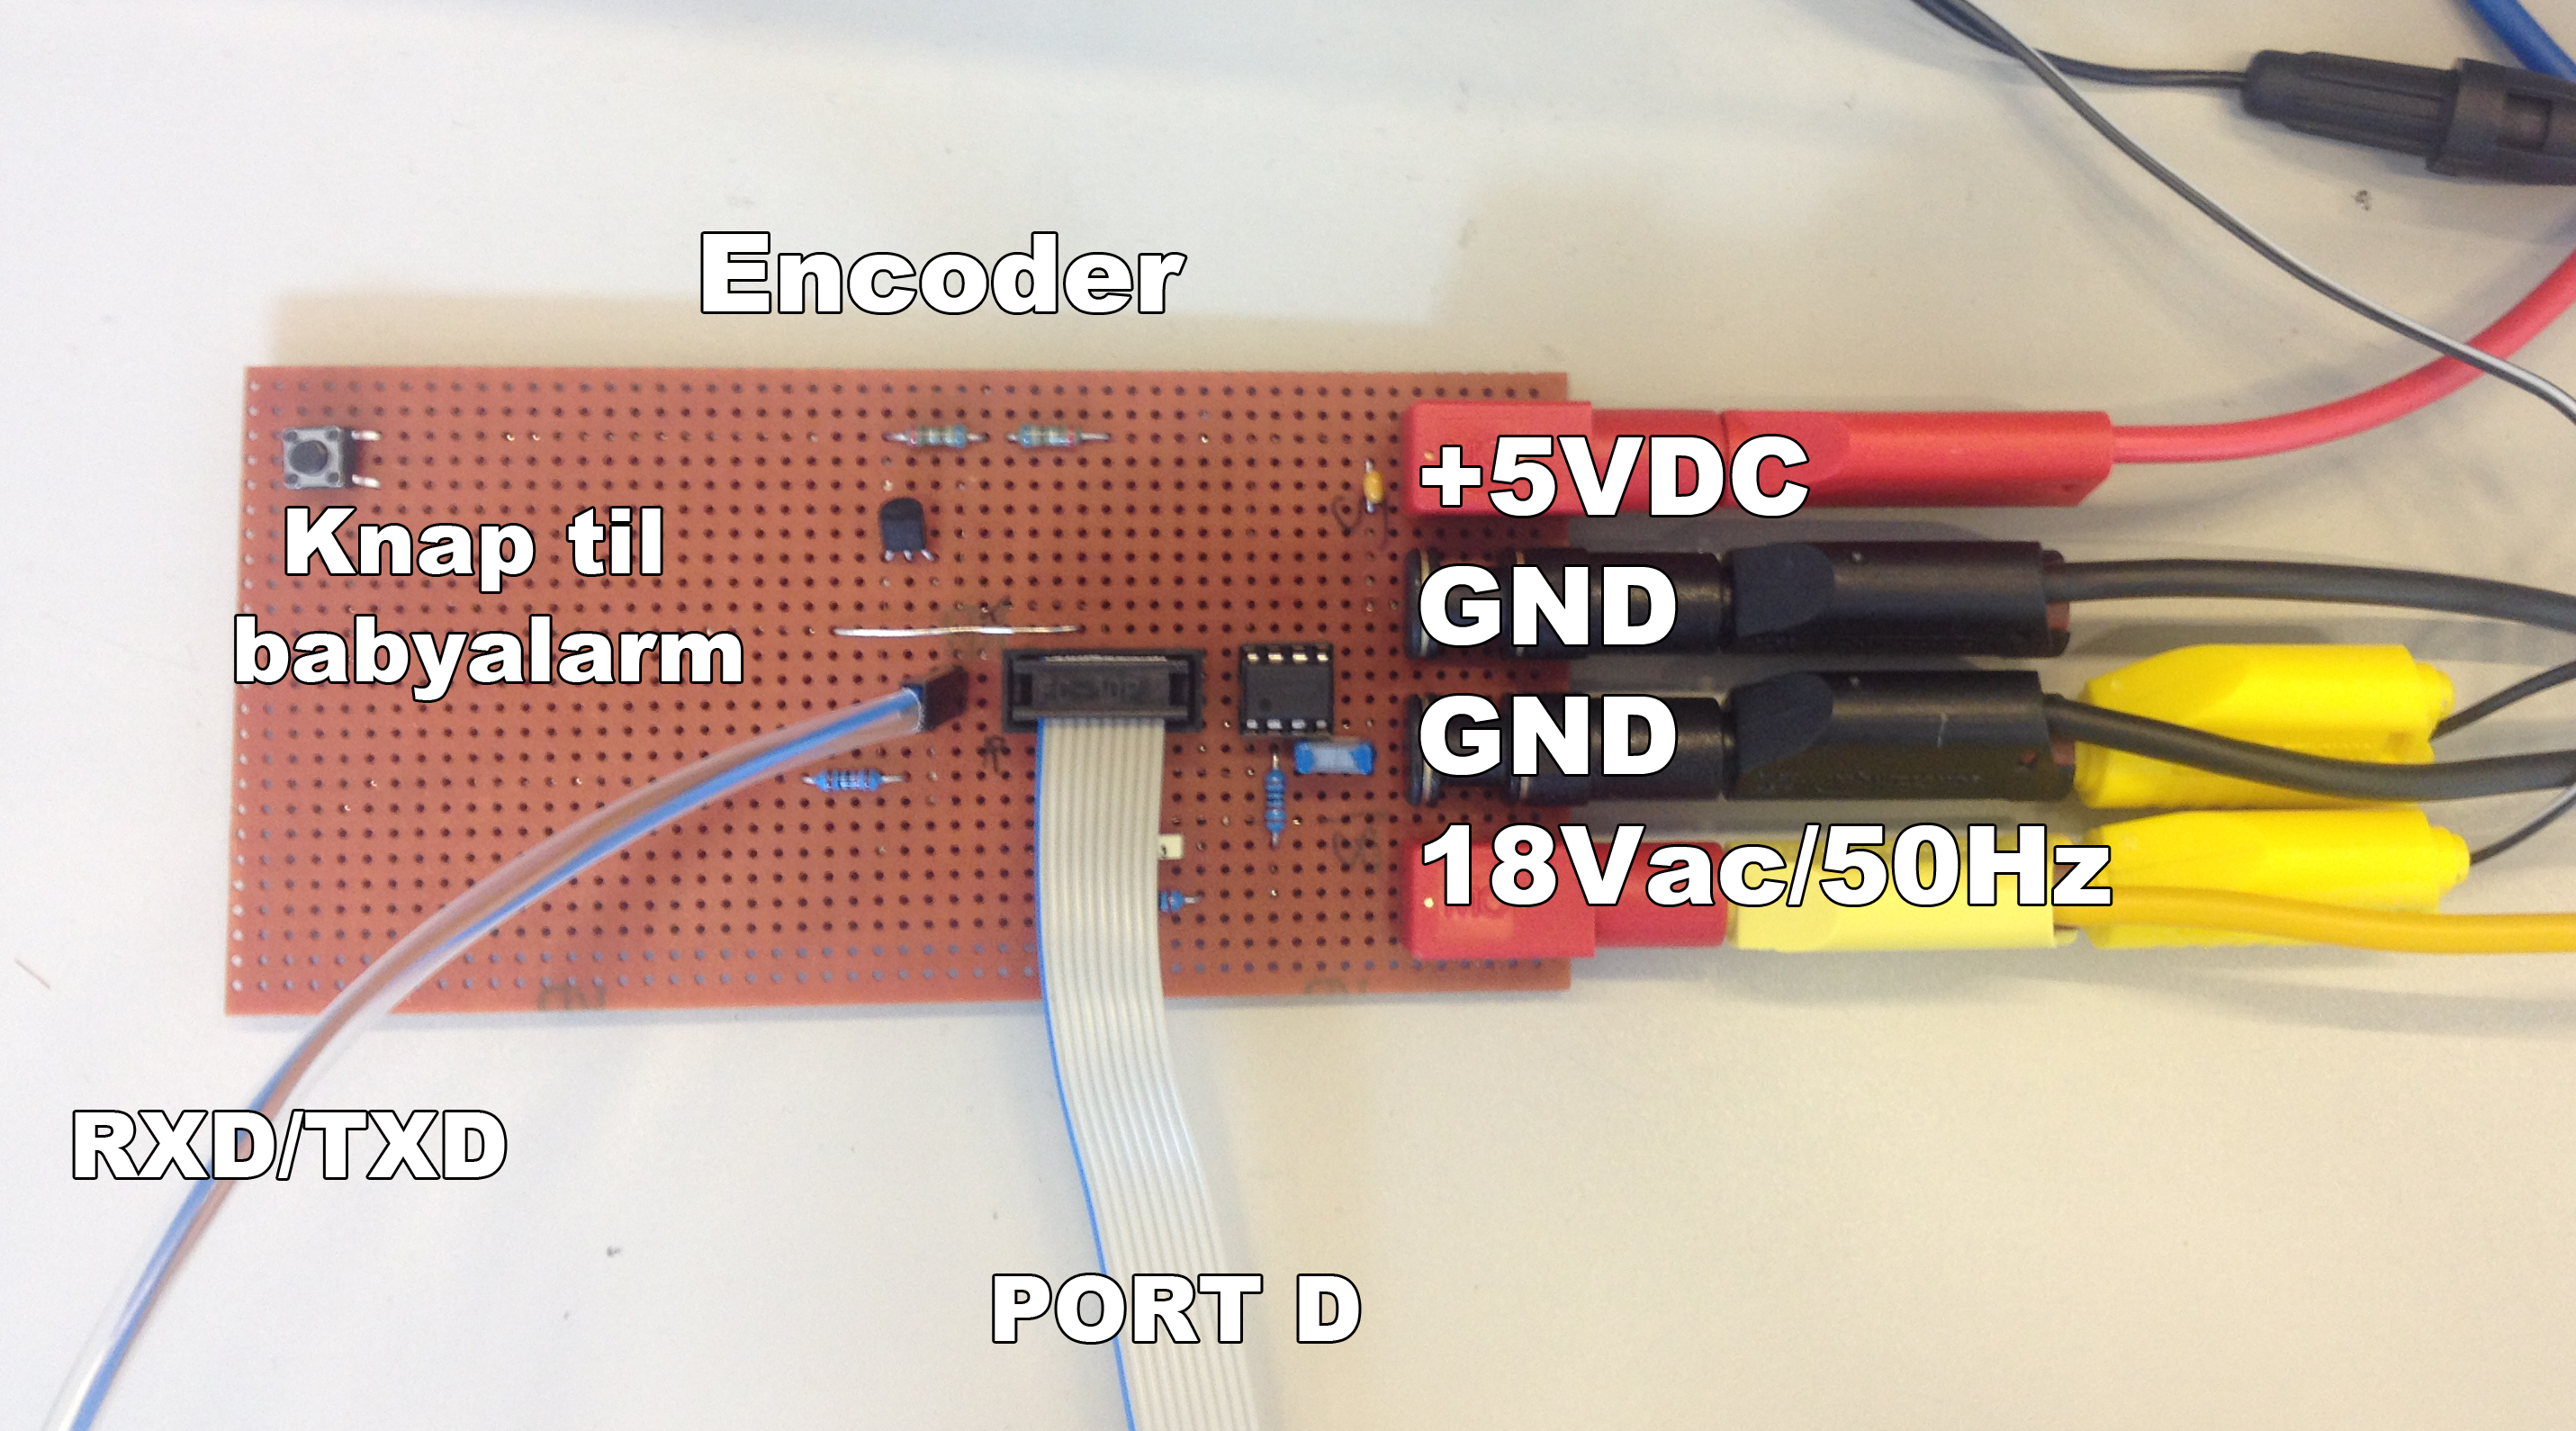
\includegraphics[width=\textwidth]{billeder/encoderveroboard}
      \caption{Encoder print}
    \label{fig:encoder_vero}
  \end{minipage}
  \hspace{0.1\textwidth}
  \begin{minipage}{0.5\textwidth}
    \centering
      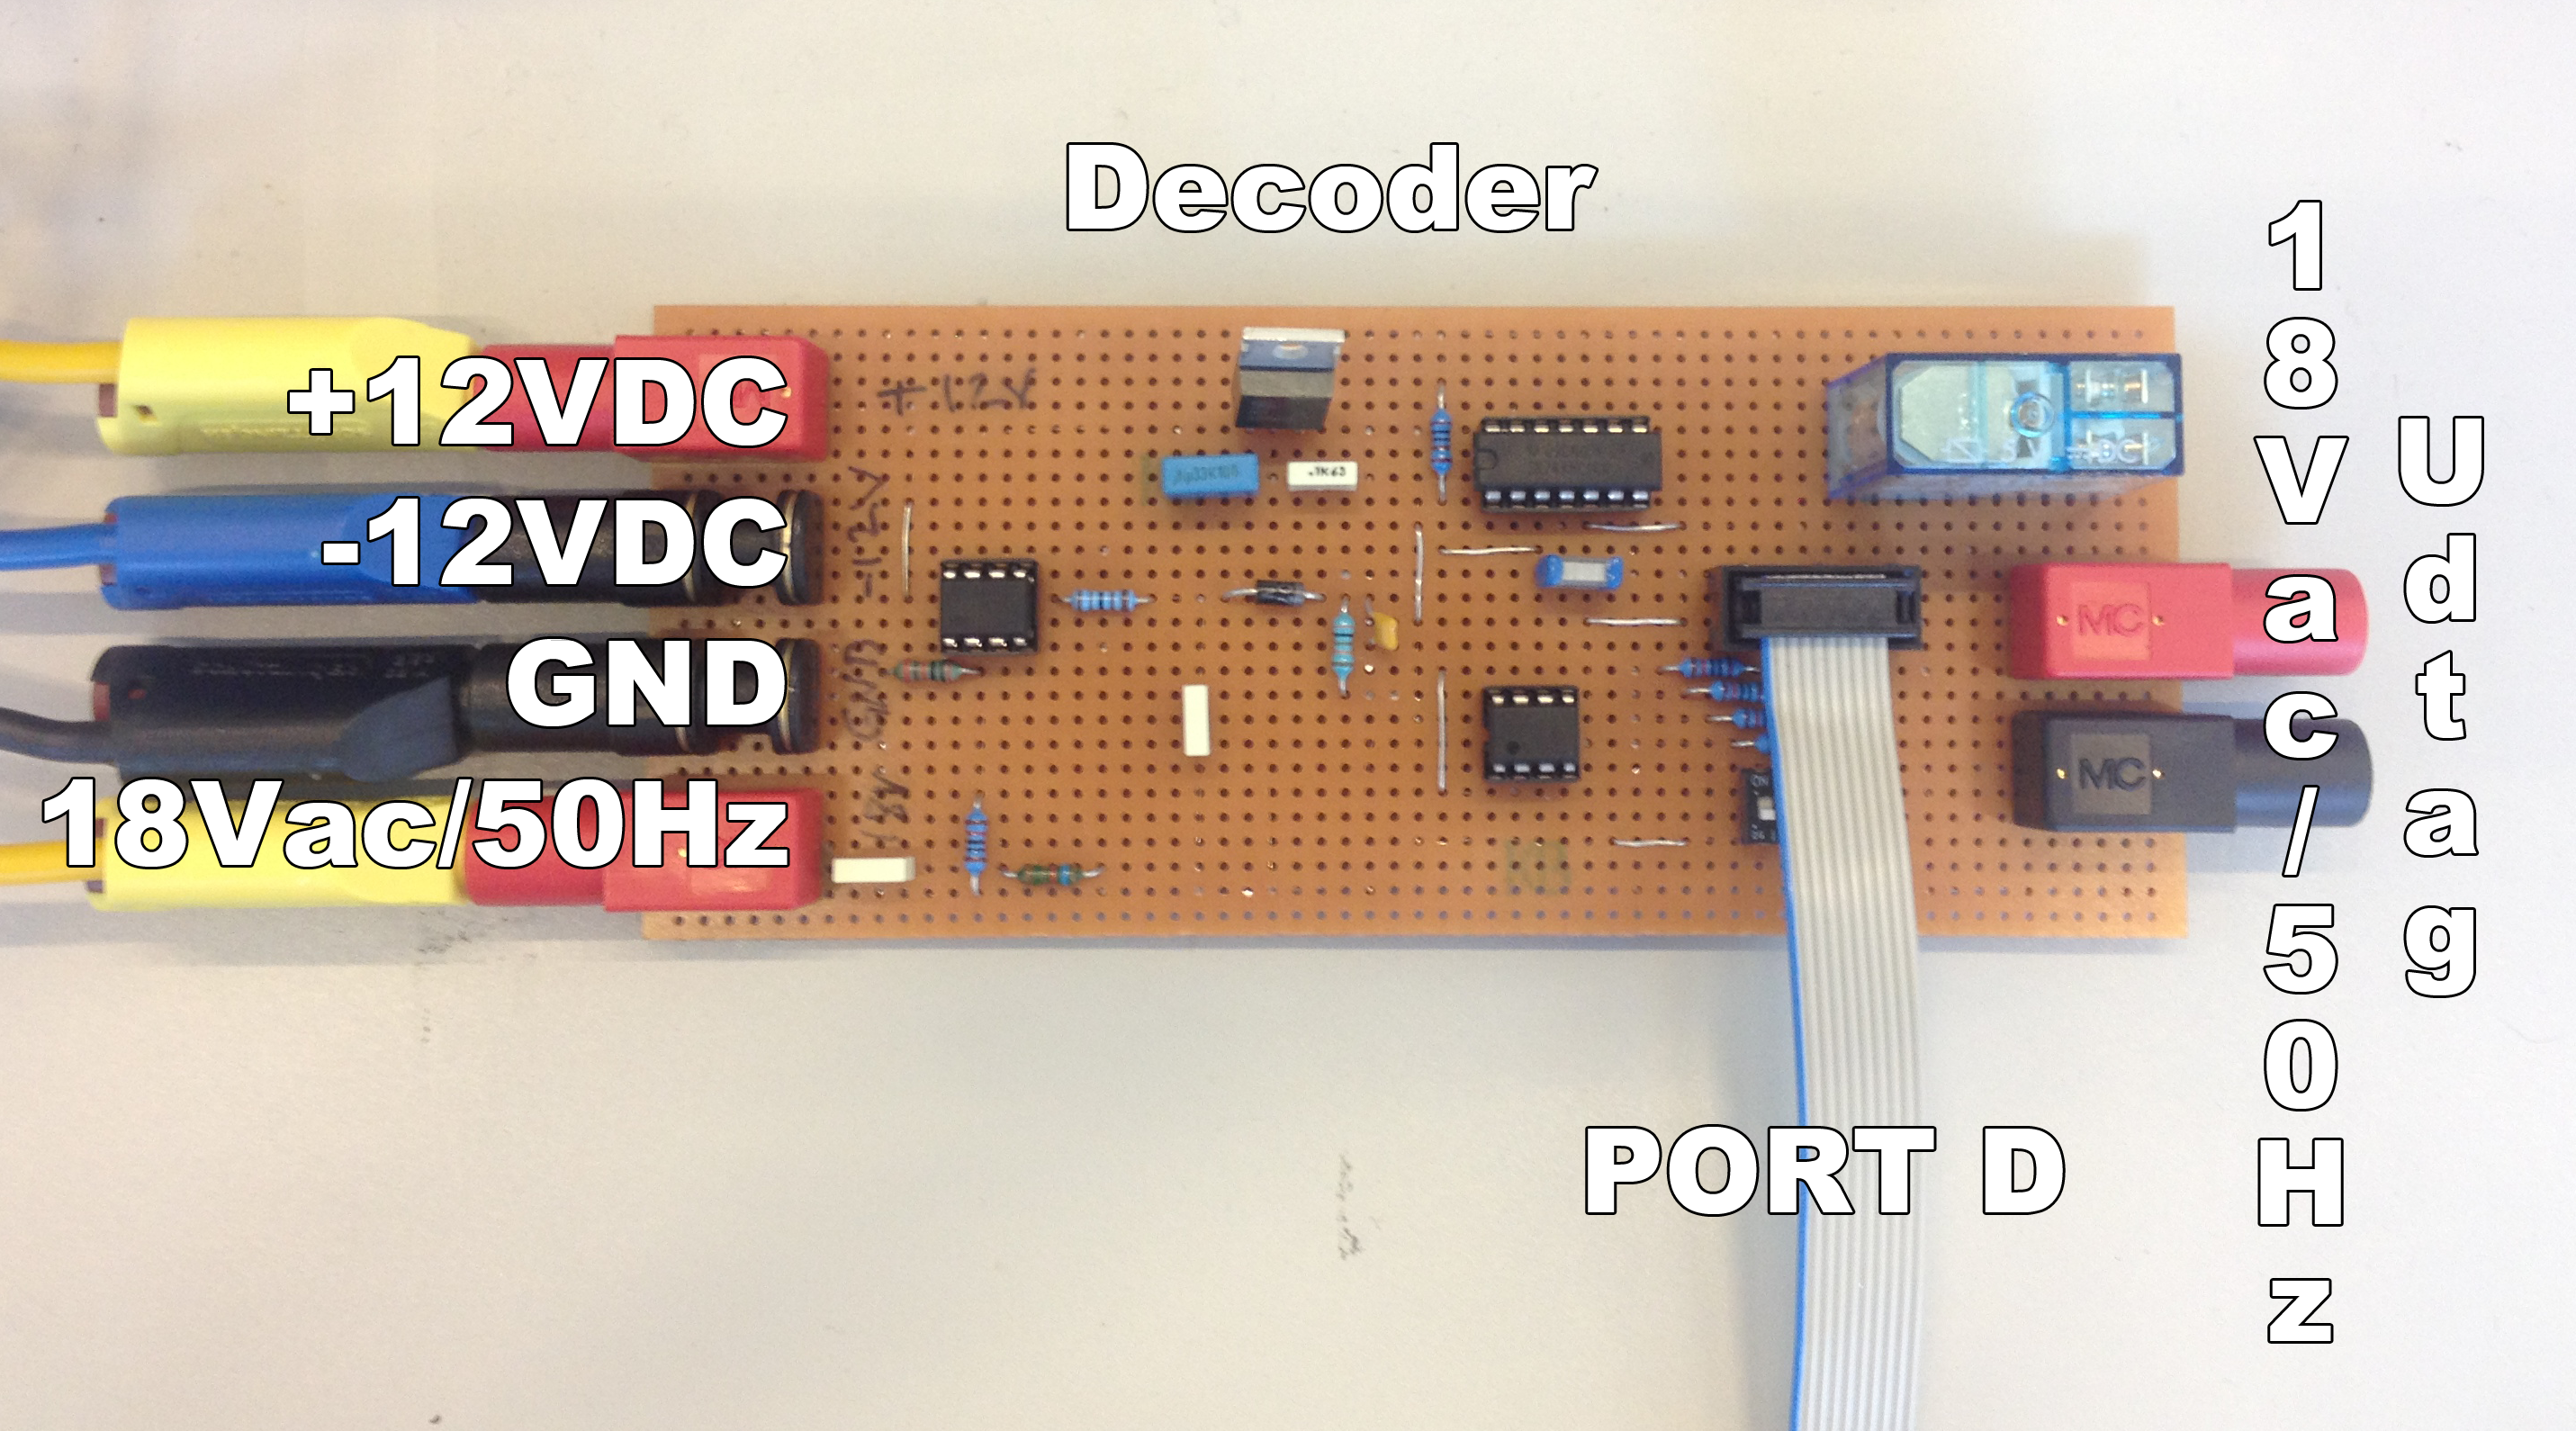
\includegraphics[width=\textwidth]{billeder/decoderveroboard}
      \caption{Decoder print}
    \label{fig:decoder_vero}
  \end{minipage}
\end{figure}

Det er ikke lykkedes at få X10-udtag softwaren til at modtage X10-bitstrømmen, derfor er der taget et scopebillede af bitstrømmen med oscilloscope indstillingen single sweep. Ses på figur \ref{fig:Scop_test}.

\begin{figure}[htbp]
  \centering
    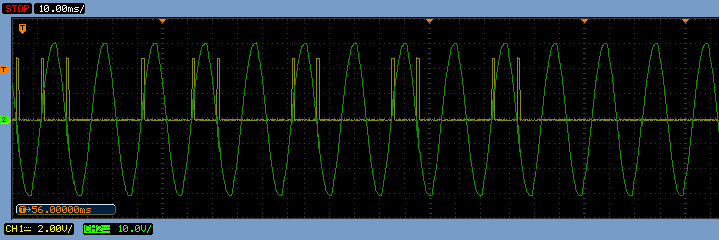
\includegraphics[width=\textwidth]{billeder/Modtager_0101_ON}
    \caption{Scopebillede af et testsignal}
    \label{fig:Scop_test}
\end{figure}

 
 
Babyalarmens advarsels SMS, kommer som en flash SMS. Dvs. SMS'en vises direkte på skærmen for brugeren, herved kan det ikke undgås at brugeren ser beskeden, når mobilen tages i brug. SMS'en som SMS-modtageren, på en iPhone, vil modtager ses herunder på figur \ref{fig:flashSMS}
 
\begin{figure}[htbp]
  \centering
    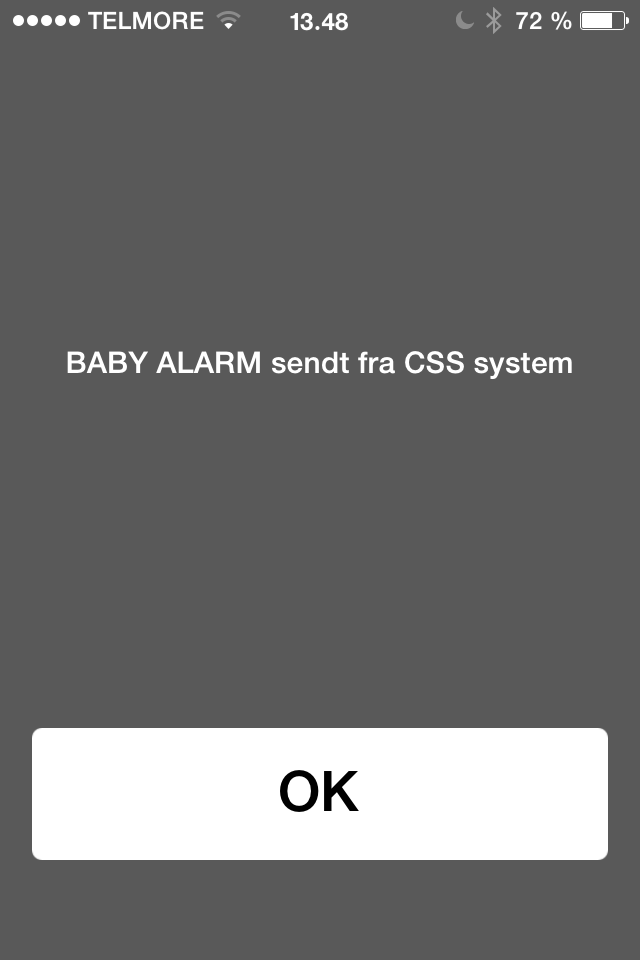
\includegraphics[width=0.4\textwidth]{billeder/flashSMS}
    \caption{Flash SMS}
    \label{fig:flashSMS}
\end{figure}
 


